
En este apartado se detalla la arquitectura de los subsistemas de análisis. Como se ha visto en el apartado anterior, el sistema se divide en dos subsistemas principales: 
\textbf{restapi} y \textbf{frontend}. El subsistema restapi contiene las clases que implementan la API REST y la lógica de negocio, mientras que el subsistema frontend abarca la interfaz de usuario.

Primero, se presentará el diagrama de paquetes para ofrecer una visión general de la estructura del sistema. Este diagrama ilustrará la organización y 
agrupación de los distintos elementos del sistema en paquetes, permitiendo una comprensión clara de su disposición y jerarquía.

A continuación, se analizará cada subsistema en detalle mediante un diagrama de componentes por cada subsistema. Se ha optado por un diagrama de componentes debido a que el sistema sigue una arquitectura MERN 
(MongoDB, Express, React, Node.js) y este tipo de diagrama aporta más valor que un diagrama de clases al reflejar más fielmente la estructura y relaciones entre los distintos módulos del sistema.

Finalmente, se describirán los componentes identificados en el diagrama, explicando su función específica dentro del sistema y las relaciones que mantienen con otros componentes. 
Esta descripción detallada permitirá entender el papel de cada componente en el funcionamiento global del sistema y cómo colaboran entre sí para cumplir con los objetivos del sistema.

Por último, una vez descritos en detalle cada subsistema, se explicará el diagrama de despliegue. Este diagrama mostrará cómo se distribuyen físicamente los componentes del sistema en el entorno de 
ejecución, especificando las configuraciones de hardware y software necesarias, así como las interconexiones entre los distintos nodos del sistema.


\subsection{Diagrama de paquetes} 
El sistema se divide en dos paquetes principales:
\begin{itemize}
    \item \textbf{restapi}: se corresponde con el \textit{backend} del sistema, contiene las clases que implementan la API REST del sistema y la lógica de negocio.
    \item \textbf{frontend}: se corresponde con el \textit{frontend} del sistema, contiene las clases que implementan la interfaz de usuario.
\end{itemize}

En la \coloredUnderline{\hyperlink{fig:6_5_Diagrama-Paquetes}{Figura \ref*{fig:6_5_Diagrama-Paquetes}: \nameref*{fig:6_5_Diagrama-Paquetes}}} se muestra el diagrama de paquetes del sistema.
\begin{figure}[H]
    \hypertarget{fig:6_5_Diagrama-Paquetes}{}
    \centering
    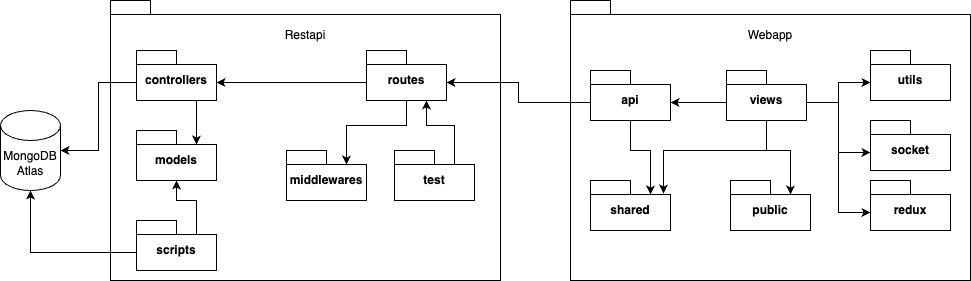
\includegraphics[width=0.8\linewidth]{figures/6-Analisis/6-Clases/6_5-vista_general-paquetes.png}
    \caption{Diagrama de Paquetes del Sistema}
    \label{fig:6_5_Diagrama-Paquetes}
\end{figure}

\subsection{Descripción de los Paquetes}
\subsubsection{restapi}
El paquete \textbf{restapi} contiene las clases que implementan la API REST del sistema y la lógica de negocio. Este paquete se divide en los siguientes subpaquetes:
\begin{itemize}
    \item \textbf{controllers}: contiene las clases que implementan los controladores de la API REST, se encargan de gestionar las peticiones HTTP y las respuestas. Se comunica con la base de datos.
    \item \textbf{models}: contiene las clases que implementan los modelos de datos del sistema.
    \item \textbf{routes}: contiene las clases que implementan las rutas de la API REST, se encargan de definir las rutas y los métodos HTTP asociados.
    \item \textbf{middlewares}: contiene las clases que implementan los middlewares de la API REST, se encargan de gestionar la autenticación y la autorización de los usuarios.
    \item \textbf{scripts}: contiene las clases que implementan los scripts de inicialización de la base de datos.
    \item \textbf{tests}: contiene las clases que implementan las pruebas unitarias de las clases de los otros subpaquetes.
\end{itemize}


\subsubsection{frontend}
El paquete \textbf{frontend} contiene los archivos que implementan la interfaz de usuario. Este paquete se divide en los siguientes subpaquetes:
\begin{itemize} 
    \item \textbf{src}: contiene los archivos que implementan la lógica de la interfaz de usuario.
    \begin{itemize}
        \item \textbf{api}: contiene los archivos que implementan la API del frontend, se encargan de gestionar las peticiones HTTP/HTTPS al backend.
        \item \textbf{views}: contiene los componentes que implementan las vistas de la interfaz de usuario. A su vez, se divide en los siguientes subpaquetes:
        \begin{itemize}
            \item \textbf{components}: contiene los archivos que implementan los componentes de la interfaz de usuario.
            \item \textbf{pages}: contiene las archivos que implementan las páginas de la interfaz de usuario.
        \end{itemize}
        \item \textbf{redux}: contiene las archivos que implementan los estados de Redux.
        \item \textbf{socket}: contiene las archivos que implementan la conexión con Socket.io.
        \item \textbf{shared}: contiene las archivos que implementan los tipos de datos compartidos entre las distintas partes de la interfaz de usuario.
        \item \textbf{utils}: contiene las archivos que implementan utilidades de la interfaz de usuario.
    \end{itemize}
    \item \textbf{public}: contiene los archivos estáticos de la interfaz de usuario.
    \item \textbf{tests}: contiene las clases que implementan las pruebas de la interfaz de usuario.
\end{itemize}

\subsection{Diagramas de Componentes}
En el estándar UML se define como componente: 
\begin{quote}
    \"Un Componente representa una parte modular de un sistema que encapsula su contenido y cuya manifestación es reemplazable dentro de su entorno.
[...]
Un Componente especifica un contrato formal de los servicios que proporciona a sus clientes y aquellos que requiere de otros Componentes o servicios en el sistema en términos de sus Interfaces proporcionadas y requeridas.
Un Componente es una unidad sustituible que puede ser reemplazada en tiempo de diseño o en tiempo de ejecución por un Componente que ofrece una funcionalidad equivalente basada en la compatibilidad de sus Interfaces. 
Siempre que el entorno sea totalmente compatible con las Interfaces proporcionadas y requeridas de un Componente, este podrá interactuar con dicho entorno."
\end{quote}

\begin{flushright}
    \cite[p. 209]{UMLomg2017}
\end{flushright}

En el contexto de este proyecto, un componente es una parte modular del sistema que encapsula su contenido y, que en un futuro, su funcionalidad podría ser ampliada o reemplazada por otra siempre que cumpla con las interfaces proporcionadas y requeridas.

\subsubsection{Diagrama de componentes del subsistema restapi}
A continuación, se presenta el diagrama de componentes del subsistema \textbf{restapi}. En este diagrama se muestran los componentes que forman parte del subsistema y las relaciones entre ellos.

    \begin{landscape}
    \begin{figure}[H]
        \hypertarget{fig:6_5_Diagrama-Componentes-restapi}{}
        \centering
        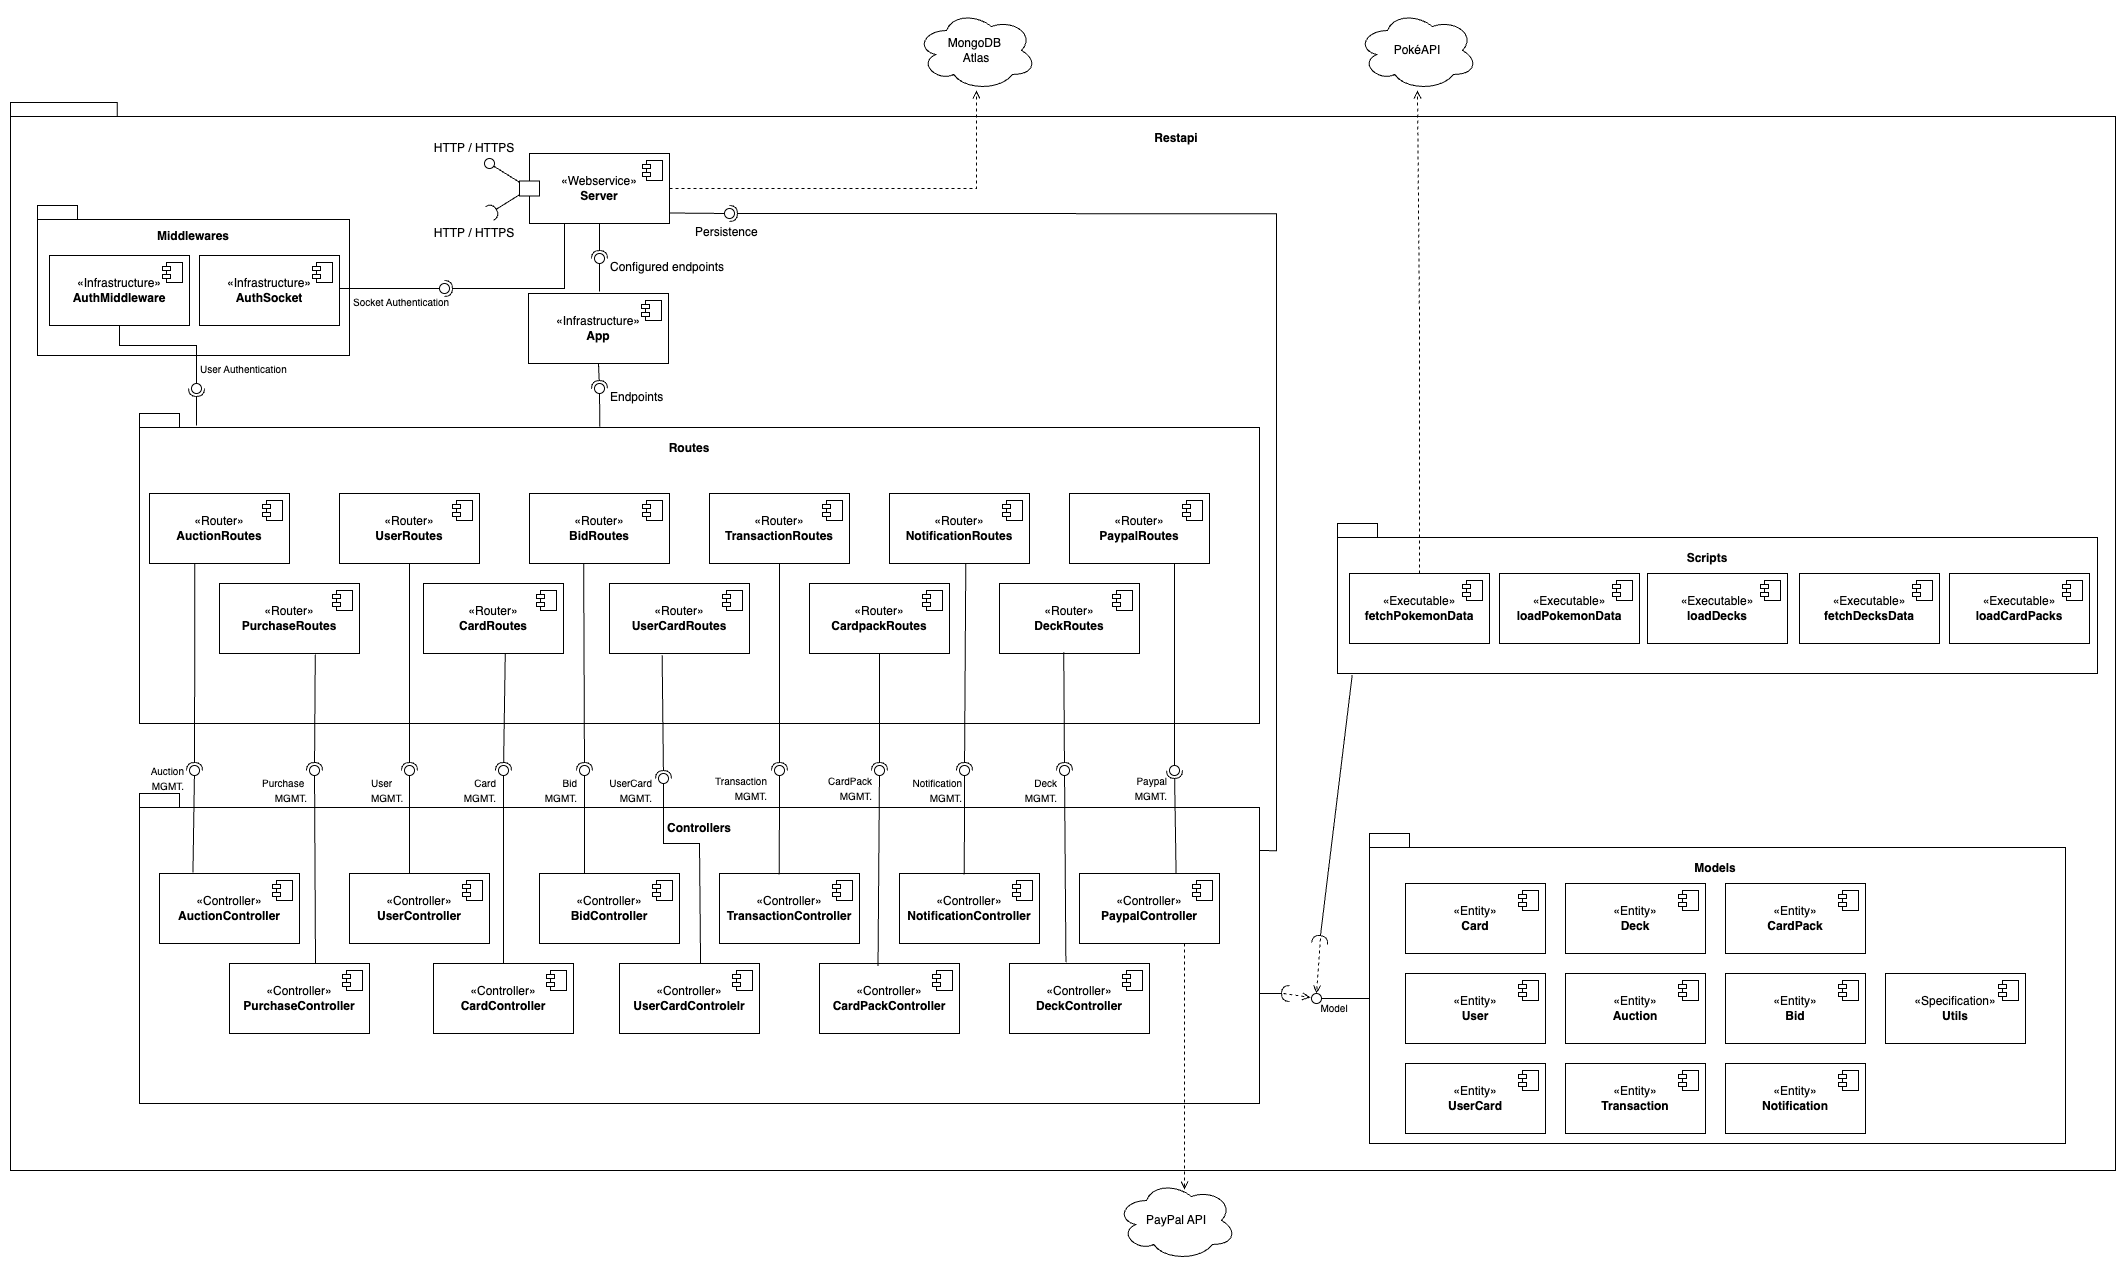
\includegraphics[width=1\linewidth]{figures/6-Analisis/6-Clases/6_5-Componentes-restapi.png}
        \caption{Diagrama de componentes del subsistema restapi}
        \label{fig:6_5_Diagrama-Componentes-restapi}
    \end{figure}
    \end{landscape}

\newpage

Por cada componente identificado en la \coloredUnderline{\hyperlink{fig:6_5_Diagrama-Componentes-restapi}{Figura \ref*{fig:6_5_Diagrama-Componentes-restapi}: \nameref*{fig:6_5_Diagrama-Componentes-restapi}}},
se ha creado una tabla con su descripción detallada, explicando su función específica dentro del sistema y las relaciones que mantiene con otros componentes.

\subsubsubsection{Descripción de componentes del subsistema restapi. \textit{Server} y \textit{App}}
%--- SERVER ---
\begin{longtable}{
    >{\columncolor{lightgreen!20}}p{4cm}
    p{12cm}
    }
    \caption{Descripción del componente:  Server} \label{table:descripcion_server} \\
    \toprule
    \rowcolor{darkgreen!50}
    \textbf{Componente} & \multicolumn{1}{>{\columncolor{darkgreen!50}\centering\arraybackslash}p{12cm}}{\textbf{SERVER}} \\
    \endfirsthead
    
    \multicolumn{2}{c}%
    {{ \tablename\ \thetable{} Descripción del componente:  Server -- continuación de la página anterior}} \\
    \toprule
    \rowcolor{darkgreen!50}
    \textbf{Componente} & \multicolumn{1}{>{\columncolor{darkgreen!50}\centering\arraybackslash}p{12cm}}{\textbf{SERVER}} \\
    \midrule
    \endhead
    
    \midrule
    \multicolumn{2}{r}{{Continúa en la siguiente página...}} \\ 
    \endfoot
    
    \bottomrule
    \endlastfoot
    
    \midrule
    Descripción & Este componente configura y gestiona los servidores HTTP y HTTPS, la conexión a MongoDB, y la gestión de conexiones de sockets mediante Socket.IO. También incluye la configuración de variables de entorno y el manejo de errores. \\
    \midrule
    Métodos & \begin{itemize}[nosep,leftmargin=*]
      \item \textbf{config()}: void, configura las variables de entorno.
      \item \textbf{createServers()}: void, crea y configura los servidores HTTP y HTTPS.
      \item \textbf{connectToDatabase()}: void, conecta a la base de datos MongoDB.
      \item \textbf{startServers()}: void, inicia los servidores HTTP y HTTPS.
      \item \textbf{setupSocketIO()}: void, configura el middleware de autenticación de sockets y maneja eventos de conexión y desconexión.
      \item \textbf{closeServer()}: Promise<void>, cierra los servidores HTTP, HTTPS y la conexión a la base de datos.
    \end{itemize} \\
    \midrule
    Interfaces requeridas & \begin{itemize}[nosep,leftmargin=*]
      \item \textbf{App}: Usa el componente App, que configura las rutas de la API REST.
      \item \textbf{AuthSocket}: Usa el middleware de autenticación de sockets.
      \item \textbf{HTTP/HTTPS}: Para la conexión a los servidores HTTP y HTTPS.
    \end{itemize} \\
    \midrule
    Interfaces proporcionadas & \begin{itemize}[nosep,leftmargin=*]
      \item \textbf{HTTP/HTTPS}: Proporciona la conexión a los servidores HTTP y HTTPS.
    \end{itemize} \\
\end{longtable}

%--- APP ---

\begin{longtable}{
    >{\columncolor{lightgreen!20}}p{4cm}
    p{12cm}
    }
    \caption{Descripción del componente:  App} \label{table:descripcion_app} \\
    \toprule
    \rowcolor{darkgreen!50}
    \textbf{Componente} & \multicolumn{1}{>{\columncolor{darkgreen!50}\centering\arraybackslash}p{12cm}}{\textbf{APP}} \\
    \endfirsthead
    
    \multicolumn{2}{c}%
    {{ \tablename\ \thetable{} Descripción del componente:  App -- continuación de la página anterior}} \\
    \toprule
    \rowcolor{darkgreen!50}
    \textbf{Componente} & \multicolumn{1}{>{\columncolor{darkgreen!50}\centering\arraybackslash}p{12cm}}{\textbf{APP}} \\
    \midrule
    \endhead
    
    \midrule
    \multicolumn{2}{r}{{Continúa en la siguiente página...}} \\ 
    \endfoot
    
    \bottomrule
    \endlastfoot
    
    \midrule
    Descripción & Este componente configura y gestiona las políticas CORS, las rutas de la API y el middleware para el manejo de errores. \\
    \midrule
    Métodos & \begin{itemize}[nosep,leftmargin=*]
      \item \textbf{use()}: void, permite configurar las rutas y los middlewares de la aplicación.
      \item \textbf{listen()}: void, inicia el servidor en el puerto especificado.
      \item \textbf{errorHandler()}: void, middleware para manejar errores en la aplicación.
    \end{itemize} \\
    \midrule
    Interfaces requeridas & \begin{itemize}[nosep,leftmargin=*]
      \item \textbf{Endpoints}: Utiliza todas las rutas de la API REST, definidas en el paquete \textit{routes}. Estas son:
        \begin{itemize}[nosep,leftmargin=*]
        \item \textbf{AuctionRouter}: Rutas que gestionan las subastas.
        \item \textbf{BidRouter}: Rutas que gestionan las pujas.
        \item \textbf{CardPackRouter}: Rutas que gestionan los sobres de cartas.
        \item \textbf{CardRouter}: Rutas que gestionan las cartas.
        \item \textbf{DeckRouter}: Rutas que gestionan los mazos de cartas.
        \item \textbf{NotificationRouter}: Rutas que gestionan las notificaciones.
        \item \textbf{PaypalRouter}: Rutas que gestionan las transacciones de PayPal.
        \item \textbf{PurchasesRouter}: Rutas que gestionan las compras.
        \item \textbf{TransactionRouter}: Rutas que gestionan las transacciones propias de la aplicación.
        \item \textbf{UserCardRouter}: Rutas que gestionan las cartas de usuario.
        \item \textbf{UserRouter}: Rutas que gestionan los usuarios.
        \end{itemize}
    \end{itemize} \\
    \midrule
    Interfaces proporcionadas & \begin{itemize}[nosep,leftmargin=*]
      \item \textbf{Configured endpoints}: Proporciona la aplicación de Express con las rutas y middlewares configurados.   
    \end{itemize} \\
\end{longtable}


%------------------------- PAQUETE MIDDLWARES -------------------------
\subsubsubsection{Descripción de componentes del subsistema restapi. Paquete \textit{middlewares}}\label{sec:descripcion_authmiddleware}
%--- AUTHMIDDLEWARE ---
\begin{longtable}{
    >{\columncolor{lightgreen!20}}p{4cm}
    p{12cm}
    }
    \caption{Descripción del componente:  AuthMiddleware} \label{table:descripcion_authmiddleware} \\
    \toprule
    \rowcolor{darkgreen!50}
    \textbf{Componente} & \multicolumn{1}{>{\columncolor{darkgreen!50}\centering\arraybackslash}p{12cm}}{\textbf{AUTHMIDDLEWARE}} \\
    \endfirsthead
    
    \multicolumn{2}{c}%
    {{ \tablename\ \thetable{} Descripción del componente:  AuthMiddleware -- continuación de la página anterior}} \\
    \toprule
    \rowcolor{darkgreen!50}
    \textbf{Componente} & \multicolumn{1}{>{\columncolor{darkgreen!50}\centering\arraybackslash}p{12cm}}{\textbf{AUTHMIDDLEWARE}} \\
    \midrule
    \endhead
    
    \midrule
    \multicolumn{2}{r}{{Continúa en la siguiente página...}} \\ 
    \endfoot
    
    \bottomrule
    \endlastfoot
    
    \midrule
    Descripción & Este componente proporciona middleware para la autenticación y autorización de usuarios mediante tokens JWT. Incluye la verificación de tokens y la verificación de roles de administrador. \\
    \midrule
    Métodos & \begin{itemize}[nosep,leftmargin=*]
      \item \textbf{auth(req: Request, res: Response, next: any)}: void, middleware para verificar la autenticidad del token JWT en las peticiones.
      \item \textbf{verifyAdmin(req: Request, res: Response, next: any)}: void, middleware para verificar que el usuario tiene rol de administrador.
    \end{itemize} \\
    \midrule
    Interfaces requeridas &  \\
    \midrule
    Interfaces proporcionadas & \begin{itemize}[nosep,leftmargin=*]
      \item \textbf{User Authentication}: Proporciona middleware para la autenticación de usuarios, verificando la validez del token JWT y, ofreciendo la posibilidad de verificar roles de administrador.
    \end{itemize} \\
    \end{longtable}

%--- AUTHSOCKET ---
\begin{longtable}{
    >{\columncolor{lightgreen!20}}p{4cm}
    p{12cm}
    }
    \caption{Descripción del componente:  AuthSocket} \label{table:descripcion_authsocket} \\
    \toprule
    \rowcolor{darkgreen!50}
    \textbf{Componente} & \multicolumn{1}{>{\columncolor{darkgreen!50}\centering\arraybackslash}p{12cm}}{\textbf{AUTHSOCKET}} \\
    \endfirsthead
    
    \multicolumn{2}{c}%
    {{ \tablename\ \thetable{} Descripción del componente:  AuthSocket -- continuación de la página anterior}} \\
    \toprule
    \rowcolor{darkgreen!50}
    \textbf{Componente} & \multicolumn{1}{>{\columncolor{darkgreen!50}\centering\arraybackslash}p{12cm}}{\textbf{AUTHSOCKET}} \\
    \midrule
    \endhead
    
    \midrule
    \multicolumn{2}{r}{{Continúa en la siguiente página...}} \\ 
    \endfoot
    
    \bottomrule
    \endlastfoot
    
    \midrule
    Descripción & Este componente proporciona el middleware para la autenticación de conexiones de sockets mediante tokens JWT. Verifica la validez y el formato del token proporcionado en el handshake de la conexión del socket. \\
    \midrule
    Métodos & \begin{itemize}[nosep,leftmargin=*]
      \item \textbf{authSocket(socket: Socket, next: (err?: Error) => void)}: void, middleware para verificar la autenticidad del token JWT en las conexiones de sockets.
    \end{itemize} \\
    \midrule
    Interfaces requeridas &  \\
    \midrule
    Interfaces proporcionadas & \begin{itemize}[nosep,leftmargin=*]
      \item \textbf{Socket Authentication}: Proporciona middleware para la autenticación de conexiones de sockets, verificando la validez del token JWT.
    \end{itemize} \\
    \end{longtable}

%------------------------- PAQUETE ROUTES -------------------------
\subsubsection{Descripción de componentes del subsistema restapi. Paquete \textit{routes}}
En el diagrama se muestra una relación de dependencia entre \textit{App} y los componentes del paquete \textit{routes}. 
En la práctica, cada componente del paquete \textit{routes} proporciona sus rutas a \textit{App} a través su propia instancia de \textit{Router} de Express. 
Se ha decidido simplificar la representación para facilitar la comprensión del diagrama, dado que todos los componentes del paquete \textit{routes} mantienen la misma relación con \textit{App}.

%--- AUCTIONROUTER ---
\begin{longtable}{
    >{\columncolor{lightgreen!20}}p{4cm}
    p{12cm}
    }
    \caption{Descripción del componente:  AuctionRouter} \label{table:descripcion_auctionrouter} \\
    \toprule
    \rowcolor{darkgreen!50}
    \textbf{Componente} & \multicolumn{1}{>{\columncolor{darkgreen!50}\centering\arraybackslash}p{12cm}}{\textbf{AUCTIONROUTER}} \\
    \endfirsthead
    
    \multicolumn{2}{c}%
    {{ \tablename\ \thetable{} Descripción del componente:  AuctionRouter -- continuación de la página anterior}} \\
    \toprule
    \rowcolor{darkgreen!50}
    \textbf{Componente} & \multicolumn{1}{>{\columncolor{darkgreen!50}\centering\arraybackslash}p{12cm}}{\textbf{AUCTIONROUTER}} \\
    \midrule
    \endhead
    
    \midrule
    \multicolumn{2}{r}{{Continúa en la siguiente página...}} \\ 
    \endfoot
    
    \bottomrule
    \endlastfoot
    
    \midrule
    Descripción & Este componente configura y gestiona las rutas relacionadas con las subastas en la aplicación Express. Incluye la autenticación mediante middleware y validaciones para las peticiones. \\
    \midrule
    Atributos & \begin{itemize}[nosep,leftmargin=*]
      \item \textbf{auctionRouter}: Router, instancia del enrutador de Express para las subastas.
    \end{itemize} \\
    \midrule
    Métodos & \begin{itemize}[nosep,leftmargin=*]
      \item \textbf{getAuctions(req: Request, res: Response)}: void, maneja la obtención de todas las subastas.
      \item \textbf{getAuction(req: Request, res: Response)}: void, maneja la obtención de una subasta por su ID.
      \item \textbf{getActiveAuctions(req: Request, res: Response)}: void, maneja la obtención de todas las subastas activas.
      \item \textbf{getActiveAuctionsByUser(req: Request, res: Response)}: void, maneja la obtención de todas las subastas activas de un usuario.
      \item \textbf{putUserCardUpForAuction(req: Request, res: Response)}: void, maneja la puesta en subasta de una carta de usuario.
      \item \textbf{withdrawnUserCardFromAuction(req: Request, res: Response)}: void, maneja la retirada de una carta de usuario de una subasta.
      \item \textbf{checkAllActiveAuctions(req: Request, res: Response)}: void, verifica todas las subastas activas y actualiza su estado si es necesario.
    \end{itemize} \\
    \midrule
    Interfaces requeridas &  \begin{itemize}[nosep,leftmargin=*]
      \item \textbf{User Authentication}: Middleware para la autenticación de usuarios.
      \item \textbf{Auction MGMT.}: Utiliza los métodos definidos en el controlador de subastas, \textit{AuctionController}.
    \end{itemize} \\
    \midrule
    Interfaces proporcionadas & \begin{itemize}[nosep,leftmargin=*]
      \item \textbf{Auction Router}: Proporciona las rutas para la gestión de subastas.
    \end{itemize} \\
    \end{longtable}

%--- BIDROUTER ---
\begin{longtable}{
    >{\columncolor{lightgreen!20}}p{4cm}
    p{12cm}
    }
    \caption{Descripción del componente:  BidRouter} \label{table:descripcion_bidrouter} \\
    \toprule
    \rowcolor{darkgreen!50}
    \textbf{Componente} & \multicolumn{1}{>{\columncolor{darkgreen!50}\centering\arraybackslash}p{12cm}}{\textbf{BIDROUTER}} \\
    \endfirsthead
    
    \multicolumn{2}{c}%
    {{ \tablename\ \thetable{} Descripción del componente:  BidRouter -- continuación de la página anterior}} \\
    \toprule
    \rowcolor{darkgreen!50}
    \textbf{Componente} & \multicolumn{1}{>{\columncolor{darkgreen!50}\centering\arraybackslash}p{12cm}}{\textbf{BIDROUTER}} \\
    \midrule
    \endhead
    
    \midrule
    \multicolumn{2}{r}{{Continúa en la siguiente página...}} \\ 
    \endfoot
    
    \bottomrule
    \endlastfoot
    
    \midrule
    Descripción & Este componente configura y gestiona las rutas relacionadas con las pujas en la aplicación Express. Incluye la autenticación mediante middleware y validaciones para las peticiones. \\
    \midrule
    Atributos & \begin{itemize}[nosep,leftmargin=*]
      \item \textbf{bidRouter}: Router, instancia del enrutador de Express para las pujas.
    \end{itemize} \\
    \midrule
    Métodos & \begin{itemize}[nosep,leftmargin=*]
      \item \textbf{getBidById(req: Request, res: Response)}: void, maneja la obtención de una puja por su ID.
      \item \textbf{createBid(req: Request, res: Response)}: void, maneja la creación de una nueva puja.
      \item \textbf{getActiveBidsByUser(req: Request, res: Response)}: void, maneja la obtención de todas las pujas activas de un usuario.
      \item \textbf{withdrawBid(req: Request, res: Response)}: void, maneja la retirada de una puja.
    \end{itemize} \\
    \midrule
    Relaciones & \begin{itemize}[nosep,leftmargin=*]
      \item \textbf{AuthMiddleware}: Middleware para la autenticación de usuarios.
      \item \textbf{BidController}: Importa y utiliza métodos del controlador de pujas.
    \end{itemize} \\
    \midrule
    Interfaces requeridas & \begin{itemize}[nosep,leftmargin=*]
      \item \textbf{User Authentication}: Middleware para la autenticación de usuarios.
      \item \textbf{Bid MGMT.}: Utiliza los métodos definidos en el controlador de pujas, \textit{BidController}.
    \end{itemize} \\
    \midrule
    Interfaces proporcionadas & \begin{itemize}[nosep,leftmargin=*]
      \item \textbf{Bid Router}: Proporciona las rutas para la gestión de pujas.
    \end{itemize} \\
    \end{longtable}

\subsubsubsection{Descripción del componente:  CardPackRouter} \label{sec:descripcion_cardpackrouter}
\begin{longtable}{
    >{\columncolor{lightgreen!20}}p{4cm}
    p{12cm}
    }
    \caption{Descripción del componente:  CardPackRouter} \label{table:descripcion_cardpackrouter} \\
    \toprule
    \rowcolor{darkgreen!50}
    \textbf{Componente} & \multicolumn{1}{>{\columncolor{darkgreen!50}\centering\arraybackslash}p{12cm}}{\textbf{CARDPACKROUTER}} \\
    \endfirsthead
    
    \multicolumn{2}{c}%
    {{ \tablename\ \thetable{} Descripción del componente:  CardPackRouter -- continuación de la página anterior}} \\
    \toprule
    \rowcolor{darkgreen!50}
    \textbf{Componente} & \multicolumn{1}{>{\columncolor{darkgreen!50}\centering\arraybackslash}p{12cm}}{\textbf{CARDPACKROUTER}} \\
    \midrule
    \endhead
    
    \midrule
    \multicolumn{2}{r}{{Continúa en la siguiente página...}} \\ 
    \endfoot
    
    \bottomrule
    \endlastfoot
    
    \midrule
    Descripción & Este componente configura y gestiona las rutas relacionadas con los sobres de cartas en la aplicación Express. Incluye la autenticación mediante middleware. \\
    \midrule
    Métodos & \begin{itemize}[nosep,leftmargin=*]
      \item \textbf{getCardPacks(req: Request, res: Response)}: void, maneja la obtención de todos los sobres de cartas.
    \end{itemize} \\
    \midrule
    Interfaces requeridas & \begin{itemize}[nosep,leftmargin=*]
      \item \textbf{User Authentication}: Middleware para la autenticación de usuarios.
      \item \textbf{CardPack MGMT.}: Utiliza los métodos definidos en el controlador de sobres de cartas, \textit{CardPackController}.
    \end{itemize} \\
    \midrule
    Interfaces proporcionadas & \begin{itemize}[nosep,leftmargin=*]
      \item \textbf{CardPack Router}: Proporciona las rutas para la gestión de sobres de cartas.
    \end{itemize} \\
    \end{longtable}


%--- CARDROUTER ---
\begin{longtable}{
    >{\columncolor{lightgreen!20}}p{4cm}
    p{12cm}
    }
    \caption{Descripción del componente:  CardRouter} \label{table:descripcion_cardrouter} \\
    \toprule
    \rowcolor{darkgreen!50}
    \textbf{Componente} & \multicolumn{1}{>{\columncolor{darkgreen!50}\centering\arraybackslash}p{12cm}}{\textbf{CARDROUTER}} \\
    \endfirsthead
    
    \multicolumn{2}{c}%
    {{ \tablename\ \thetable{} Descripción del componente:  CardRouter -- continuación de la página anterior}} \\
    \toprule
    \rowcolor{darkgreen!50}
    \textbf{Componente} & \multicolumn{1}{>{\columncolor{darkgreen!50}\centering\arraybackslash}p{12cm}}{\textbf{CARDROUTER}} \\
    \midrule
    \endhead
    
    \midrule
    \multicolumn{2}{r}{{Continúa en la siguiente página...}} \\ 
    \endfoot
    
    \bottomrule
    \endlastfoot
    
    \midrule
    Descripción & Esta clase configura y gestiona las rutas relacionadas con las cartas en la aplicación Express. Incluye la autenticación mediante middleware y validaciones para las peticiones. \\
    \midrule
    Métodos & \begin{itemize}[nosep,leftmargin=*]
      \item \textbf{getCard(req: Request, res: Response)}: void, maneja la obtención de una carta por su ID.
    \end{itemize} \\
    \midrule
    Interfaces requeridas  & \begin{itemize}[nosep,leftmargin=*]
      \item \textbf{User Authentication}: Middleware para la autenticación de usuarios.
      \item \textbf{Card MGMT.}: Utiliza los métodos definidos en el controlador de cartas, \textit{CardController}.
    \end{itemize} \\
    \midrule
    Interfaces proporcionadas & \begin{itemize}[nosep,leftmargin=*]
        \item \textbf{Card Router}: Proporciona las rutas para la gestión de cartas.
    \end{itemize} \\
    \end{longtable}

% --- NOTIFICATIONROUTER ---
\begin{longtable}{
    >{\columncolor{lightgreen!20}}p{4cm}
    p{12cm}
    }
    \caption{Descripción del componente:  NotificationRouter} \label{table:descripcion_notificationrouter} \\
    \toprule
    \rowcolor{darkgreen!50}
    \textbf{Componente} & \multicolumn{1}{>{\columncolor{darkgreen!50}\centering\arraybackslash}p{12cm}}{\textbf{NOTIFICATIONROUTER}} \\
    \endfirsthead
    
    \multicolumn{2}{c}%
    {{ \tablename\ \thetable{} Descripción del componente:  NotificationRouter -- continuación de la página anterior}} \\
    \toprule
    \rowcolor{darkgreen!50}
    \textbf{Componente} & \multicolumn{1}{>{\columncolor{darkgreen!50}\centering\arraybackslash}p{12cm}}{\textbf{NOTIFICATIONROUTER}} \\
    \midrule
    \endhead
    
    \midrule
    \multicolumn{2}{r}{{Continúa en la siguiente página...}} \\ 
    \endfoot
    
    \bottomrule
    \endlastfoot
    
    \midrule
    Descripción & Este componente configura y gestiona las rutas relacionadas con las notificaciones en la aplicación Express. Incluye la autenticación mediante middleware y validaciones para las peticiones. \\
    \midrule
    Atributos & \begin{itemize}[nosep,leftmargin=*]
      \item \textbf{notificationRouter}: Router, instancia del enrutador de Express para las notificaciones.
    \end{itemize} \\
    \midrule
    Métodos & \begin{itemize}[nosep,leftmargin=*]
      \item \textbf{getNotifications(req: Request, res: Response)}: void, maneja la obtención de todas las notificaciones de un usuario.
      \item \textbf{markAsRead(req: Request, res: Response)}: void, maneja el marcado de una notificación como leída.
      \item \textbf{markAllAsRead(req: Request, res: Response)}: void, maneja el marcado de todas las notificaciones de un usuario como leídas.
      \item \textbf{hasUnreadNotifications(req: Request, res: Response)}: void, verifica si un usuario tiene notificaciones no leídas.
    \end{itemize} \\
    \midrule
    Interfaces requeridas & \begin{itemize}[nosep,leftmargin=*]
      \item \textbf{User Authentication}: Middleware para la autenticación de usuarios.
      \item \textbf{Notification MGMT.}: Utiliza los métodos definidos en el controlador de notificaciones, \textit{NotificationController}.
    \end{itemize} \\
    \midrule
    Interfaces proporcionadas & \begin{itemize}[nosep,leftmargin=*]
        \item \textbf{Notification Router}: Proporciona las rutas para la gestión de notificaciones.
    \end{itemize} \\
    \end{longtable}

%--- PAYPALROUTER ---
\begin{longtable}{
    >{\columncolor{lightgreen!20}}p{4cm}
    p{12cm}
    }
    \caption{Descripción del componente:  PaypalRouter} \label{table:descripcion_paypalrouter} \\
    \toprule
    \rowcolor{darkgreen!50}
    \textbf{Componente} & \multicolumn{1}{>{\columncolor{darkgreen!50}\centering\arraybackslash}p{12cm}}{\textbf{PAYPALROUTER}} \\
    \endfirsthead
    
    \multicolumn{2}{c}%
    {{ \tablename\ \thetable{} Descripción del componente:  PaypalRouter -- continuación de la página anterior}} \\
    \toprule
    \rowcolor{darkgreen!50}
    \textbf{Componente} & \multicolumn{1}{>{\columncolor{darkgreen!50}\centering\arraybackslash}p{12cm}}{\textbf{PAYPALROUTER}} \\
    \midrule
    \endhead
    
    \midrule
    \multicolumn{2}{r}{{Continúa en la siguiente página...}} \\ 
    \endfoot
    
    \bottomrule
    \endlastfoot
    
    \midrule
    Descripción & Este componente configura y gestiona las rutas relacionadas con las órdenes de PayPal en la aplicación Express. Incluye validaciones para las peticiones y manejo de errores. \\
    \midrule
    Métodos & \begin{itemize}[nosep,leftmargin=*]
      \item \textbf{createOrder(req: Request, res: Response)}: void, maneja la creación de una nueva orden de PayPal.
      \item \textbf{updateOrder(req: Request, res: Response)}: void, maneja la actualización del saldo de un usuario después de completar un pago.
    \end{itemize} \\
    \midrule
    Interfaces requeridas & \begin{itemize}[nosep,leftmargin=*]
      \item \textbf{Paypal MGMT.}: Utiliza los métodos definidos en el controlador de PayPal, \textit{PaypalController}.
    \end{itemize} \\
    \midrule
    Interfaces proporcionadas & \begin{itemize}[nosep,leftmargin=*]
      \item \textbf{Paypal Router}: Proporciona las rutas para la gestión de órdenes de PayPal.
    \end{itemize} \\
    \end{longtable}

%------------------------- PAQUETE CONTROLLERS -------------------------


\subsubsubsection{Descripción de los Componentes del Subsistema restapi}


\subsubsection{frontend}
A continuación, se presenta el diagrama de componentes del subsistema \textbf{frontend}. En este diagrama se muestran los componentes que forman parte del subsistema y las relaciones entre ellos.
